\documentclass[border=3pt]{standalone}
% Preâmbulo compartilhado pelos diagramas TikZ da aula 7 de Navegação (Implementação do A*)
\usepackage[T1]{fontenc}
\usepackage[utf8]{inputenc}
\usepackage{lmodern}
\usepackage{amsmath}
\usepackage{xcolor}
\usepackage{tikz}
\usetikzlibrary{arrows.meta,angles,quotes,decorations.pathmorphing,decorations.pathreplacing,calc,
                positioning,shapes.geometric,shapes.misc,backgrounds,fit,
                math}

% Paleta (mesma dos SVGs originais)
\definecolor{dblue}{HTML}{2A5B8C}
\definecolor{dorange}{HTML}{B3541E}
\definecolor{dgreen}{HTML}{4A7C59}
\definecolor{dred}{HTML}{9C4B4B}
\definecolor{dcream}{HTML}{F4F1EA}
\definecolor{dshade}{HTML}{DDD7C9}

% Função gaussiana (não normalizada por padrão de escala visual)
\pgfmathdeclarefunction{gauss}{3}{%
  \pgfmathparse{1/(#3*sqrt(2*pi))*exp(-((#1-#2)^2)/(2*#3^2))}%
}

% Estilos comuns (prefixo d... para não colidir com chaves internas do pgf)
\tikzset{
  >={Stealth[length=2mm]},
  dguide/.style={gray!55, dashed, line width=0.4pt},
  daxis/.style={gray!60, line width=0.7pt, ->},
  dbody/.style={fill=black!3, draw=black!80, line width=1pt},
  dacc/.style={draw=dblue, line width=1pt},
  dlbl/.style={black!55, font=\small},
  dsub/.style={black!45, font=\footnotesize},
  dstate/.style={circle, draw=black!80, fill=dcream, line width=1pt,
                 minimum size=17mm, font=\large, inner sep=1pt},
  dobs/.style={circle, draw=black!80, fill=dshade, line width=1pt,
               minimum size=14mm, font=\large, inner sep=1pt},
  dbox/.style={rounded corners=2pt, draw=black!80, fill=dcream, line width=1pt,
               align=center, inner sep=6pt},
  dop/.style={circle, draw=black!80, fill=white, line width=1pt,
              minimum size=6mm, inner sep=0pt, font=\small},
  dtrans/.style={->, dblue, line width=1pt},
  dmeas/.style={->, dorange, line width=1pt},
  dcurve/.style={line width=1pt, dblue},
  dcurveb/.style={line width=1.4pt, dorange},
}

\begin{document}
\hyphenpenalty=10000 \exhyphenpenalty=10000 \tolerance=9999 \emergencystretch=3em
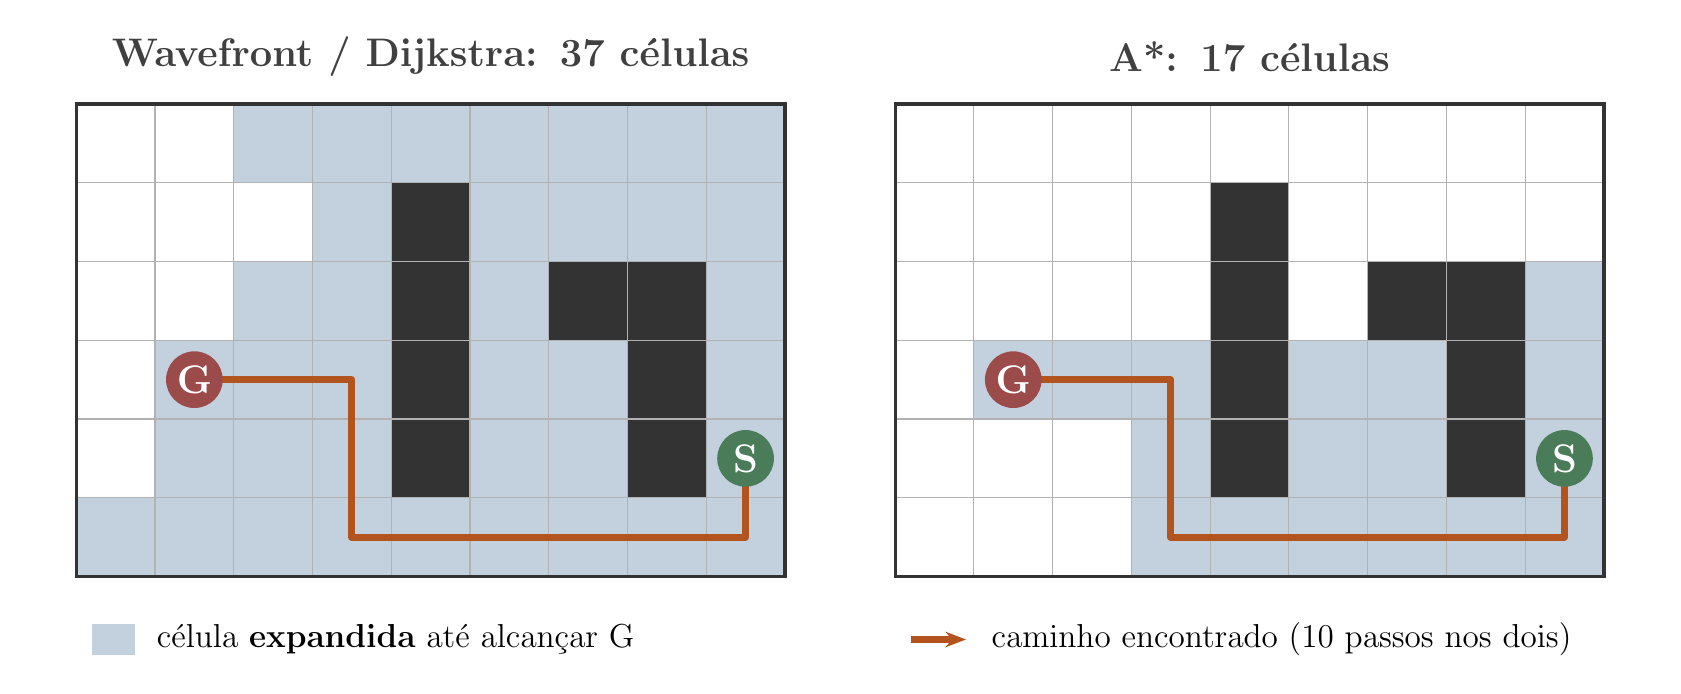
\begin{tikzpicture}[x=1cm,y=1cm]
\draw[fill=white, draw=black!30, line width=0.4pt] (0.000,5.000) rectangle ++(1.000,1.000);
\draw[fill=white, draw=black!30, line width=0.4pt] (1.000,5.000) rectangle ++(1.000,1.000);
\draw[fill=dblue!28!white, draw=black!30, line width=0.4pt] (2.000,5.000) rectangle ++(1.000,1.000);
\draw[fill=dblue!28!white, draw=black!30, line width=0.4pt] (3.000,5.000) rectangle ++(1.000,1.000);
\draw[fill=dblue!28!white, draw=black!30, line width=0.4pt] (4.000,5.000) rectangle ++(1.000,1.000);
\draw[fill=dblue!28!white, draw=black!30, line width=0.4pt] (5.000,5.000) rectangle ++(1.000,1.000);
\draw[fill=dblue!28!white, draw=black!30, line width=0.4pt] (6.000,5.000) rectangle ++(1.000,1.000);
\draw[fill=dblue!28!white, draw=black!30, line width=0.4pt] (7.000,5.000) rectangle ++(1.000,1.000);
\draw[fill=dblue!28!white, draw=black!30, line width=0.4pt] (8.000,5.000) rectangle ++(1.000,1.000);
\draw[fill=white, draw=black!30, line width=0.4pt] (0.000,4.000) rectangle ++(1.000,1.000);
\draw[fill=white, draw=black!30, line width=0.4pt] (1.000,4.000) rectangle ++(1.000,1.000);
\draw[fill=white, draw=black!30, line width=0.4pt] (2.000,4.000) rectangle ++(1.000,1.000);
\draw[fill=dblue!28!white, draw=black!30, line width=0.4pt] (3.000,4.000) rectangle ++(1.000,1.000);
\draw[fill=black!80, draw=black!30, line width=0.4pt] (4.000,4.000) rectangle ++(1.000,1.000);
\draw[fill=dblue!28!white, draw=black!30, line width=0.4pt] (5.000,4.000) rectangle ++(1.000,1.000);
\draw[fill=dblue!28!white, draw=black!30, line width=0.4pt] (6.000,4.000) rectangle ++(1.000,1.000);
\draw[fill=dblue!28!white, draw=black!30, line width=0.4pt] (7.000,4.000) rectangle ++(1.000,1.000);
\draw[fill=dblue!28!white, draw=black!30, line width=0.4pt] (8.000,4.000) rectangle ++(1.000,1.000);
\draw[fill=white, draw=black!30, line width=0.4pt] (0.000,3.000) rectangle ++(1.000,1.000);
\draw[fill=white, draw=black!30, line width=0.4pt] (1.000,3.000) rectangle ++(1.000,1.000);
\draw[fill=dblue!28!white, draw=black!30, line width=0.4pt] (2.000,3.000) rectangle ++(1.000,1.000);
\draw[fill=dblue!28!white, draw=black!30, line width=0.4pt] (3.000,3.000) rectangle ++(1.000,1.000);
\draw[fill=black!80, draw=black!30, line width=0.4pt] (4.000,3.000) rectangle ++(1.000,1.000);
\draw[fill=dblue!28!white, draw=black!30, line width=0.4pt] (5.000,3.000) rectangle ++(1.000,1.000);
\draw[fill=black!80, draw=black!30, line width=0.4pt] (6.000,3.000) rectangle ++(1.000,1.000);
\draw[fill=black!80, draw=black!30, line width=0.4pt] (7.000,3.000) rectangle ++(1.000,1.000);
\draw[fill=dblue!28!white, draw=black!30, line width=0.4pt] (8.000,3.000) rectangle ++(1.000,1.000);
\draw[fill=white, draw=black!30, line width=0.4pt] (0.000,2.000) rectangle ++(1.000,1.000);
\draw[fill=dblue!28!white, draw=black!30, line width=0.4pt] (1.000,2.000) rectangle ++(1.000,1.000);
\draw[fill=dblue!28!white, draw=black!30, line width=0.4pt] (2.000,2.000) rectangle ++(1.000,1.000);
\draw[fill=dblue!28!white, draw=black!30, line width=0.4pt] (3.000,2.000) rectangle ++(1.000,1.000);
\draw[fill=black!80, draw=black!30, line width=0.4pt] (4.000,2.000) rectangle ++(1.000,1.000);
\draw[fill=dblue!28!white, draw=black!30, line width=0.4pt] (5.000,2.000) rectangle ++(1.000,1.000);
\draw[fill=dblue!28!white, draw=black!30, line width=0.4pt] (6.000,2.000) rectangle ++(1.000,1.000);
\draw[fill=black!80, draw=black!30, line width=0.4pt] (7.000,2.000) rectangle ++(1.000,1.000);
\draw[fill=dblue!28!white, draw=black!30, line width=0.4pt] (8.000,2.000) rectangle ++(1.000,1.000);
\draw[fill=white, draw=black!30, line width=0.4pt] (0.000,1.000) rectangle ++(1.000,1.000);
\draw[fill=dblue!28!white, draw=black!30, line width=0.4pt] (1.000,1.000) rectangle ++(1.000,1.000);
\draw[fill=dblue!28!white, draw=black!30, line width=0.4pt] (2.000,1.000) rectangle ++(1.000,1.000);
\draw[fill=dblue!28!white, draw=black!30, line width=0.4pt] (3.000,1.000) rectangle ++(1.000,1.000);
\draw[fill=black!80, draw=black!30, line width=0.4pt] (4.000,1.000) rectangle ++(1.000,1.000);
\draw[fill=dblue!28!white, draw=black!30, line width=0.4pt] (5.000,1.000) rectangle ++(1.000,1.000);
\draw[fill=dblue!28!white, draw=black!30, line width=0.4pt] (6.000,1.000) rectangle ++(1.000,1.000);
\draw[fill=black!80, draw=black!30, line width=0.4pt] (7.000,1.000) rectangle ++(1.000,1.000);
\draw[fill=dblue!28!white, draw=black!30, line width=0.4pt] (8.000,1.000) rectangle ++(1.000,1.000);
\draw[fill=dblue!28!white, draw=black!30, line width=0.4pt] (0.000,0.000) rectangle ++(1.000,1.000);
\draw[fill=dblue!28!white, draw=black!30, line width=0.4pt] (1.000,0.000) rectangle ++(1.000,1.000);
\draw[fill=dblue!28!white, draw=black!30, line width=0.4pt] (2.000,0.000) rectangle ++(1.000,1.000);
\draw[fill=dblue!28!white, draw=black!30, line width=0.4pt] (3.000,0.000) rectangle ++(1.000,1.000);
\draw[fill=dblue!28!white, draw=black!30, line width=0.4pt] (4.000,0.000) rectangle ++(1.000,1.000);
\draw[fill=dblue!28!white, draw=black!30, line width=0.4pt] (5.000,0.000) rectangle ++(1.000,1.000);
\draw[fill=dblue!28!white, draw=black!30, line width=0.4pt] (6.000,0.000) rectangle ++(1.000,1.000);
\draw[fill=dblue!28!white, draw=black!30, line width=0.4pt] (7.000,0.000) rectangle ++(1.000,1.000);
\draw[fill=dblue!28!white, draw=black!30, line width=0.4pt] (8.000,0.000) rectangle ++(1.000,1.000);
\draw[black!80, line width=1.2pt] (0.000,0.000) rectangle (9.000,6.000);
\draw[dorange, line width=2.6pt, line cap=round, line join=round, -{Stealth[length=3.0mm]}] (8.500,1.500) -- (8.500,0.500) -- (7.500,0.500) -- (6.500,0.500) -- (5.500,0.500) -- (4.500,0.500) -- (3.500,0.500) -- (3.500,1.500) -- (3.500,2.500) -- (2.500,2.500) -- (1.500,2.500);
\node[circle, fill=dgreen, text=white, font=\bfseries\Large, inner sep=1pt, minimum size=0.72cm] at (8.500,1.500) {S};
\node[circle, fill=dred, text=white, font=\bfseries\Large, inner sep=1pt, minimum size=0.72cm] at (1.500,2.500) {G};
\node[font=\Large\bfseries, black!75, text width=10.0cm, align=center] at (4.500,6.600) {Wavefront / Dijkstra: 37 células};
\draw[fill=white, draw=black!30, line width=0.4pt] (10.400,5.000) rectangle ++(1.000,1.000);
\draw[fill=white, draw=black!30, line width=0.4pt] (11.400,5.000) rectangle ++(1.000,1.000);
\draw[fill=white, draw=black!30, line width=0.4pt] (12.400,5.000) rectangle ++(1.000,1.000);
\draw[fill=white, draw=black!30, line width=0.4pt] (13.400,5.000) rectangle ++(1.000,1.000);
\draw[fill=white, draw=black!30, line width=0.4pt] (14.400,5.000) rectangle ++(1.000,1.000);
\draw[fill=white, draw=black!30, line width=0.4pt] (15.400,5.000) rectangle ++(1.000,1.000);
\draw[fill=white, draw=black!30, line width=0.4pt] (16.400,5.000) rectangle ++(1.000,1.000);
\draw[fill=white, draw=black!30, line width=0.4pt] (17.400,5.000) rectangle ++(1.000,1.000);
\draw[fill=white, draw=black!30, line width=0.4pt] (18.400,5.000) rectangle ++(1.000,1.000);
\draw[fill=white, draw=black!30, line width=0.4pt] (10.400,4.000) rectangle ++(1.000,1.000);
\draw[fill=white, draw=black!30, line width=0.4pt] (11.400,4.000) rectangle ++(1.000,1.000);
\draw[fill=white, draw=black!30, line width=0.4pt] (12.400,4.000) rectangle ++(1.000,1.000);
\draw[fill=white, draw=black!30, line width=0.4pt] (13.400,4.000) rectangle ++(1.000,1.000);
\draw[fill=black!80, draw=black!30, line width=0.4pt] (14.400,4.000) rectangle ++(1.000,1.000);
\draw[fill=white, draw=black!30, line width=0.4pt] (15.400,4.000) rectangle ++(1.000,1.000);
\draw[fill=white, draw=black!30, line width=0.4pt] (16.400,4.000) rectangle ++(1.000,1.000);
\draw[fill=white, draw=black!30, line width=0.4pt] (17.400,4.000) rectangle ++(1.000,1.000);
\draw[fill=white, draw=black!30, line width=0.4pt] (18.400,4.000) rectangle ++(1.000,1.000);
\draw[fill=white, draw=black!30, line width=0.4pt] (10.400,3.000) rectangle ++(1.000,1.000);
\draw[fill=white, draw=black!30, line width=0.4pt] (11.400,3.000) rectangle ++(1.000,1.000);
\draw[fill=white, draw=black!30, line width=0.4pt] (12.400,3.000) rectangle ++(1.000,1.000);
\draw[fill=white, draw=black!30, line width=0.4pt] (13.400,3.000) rectangle ++(1.000,1.000);
\draw[fill=black!80, draw=black!30, line width=0.4pt] (14.400,3.000) rectangle ++(1.000,1.000);
\draw[fill=white, draw=black!30, line width=0.4pt] (15.400,3.000) rectangle ++(1.000,1.000);
\draw[fill=black!80, draw=black!30, line width=0.4pt] (16.400,3.000) rectangle ++(1.000,1.000);
\draw[fill=black!80, draw=black!30, line width=0.4pt] (17.400,3.000) rectangle ++(1.000,1.000);
\draw[fill=dblue!28!white, draw=black!30, line width=0.4pt] (18.400,3.000) rectangle ++(1.000,1.000);
\draw[fill=white, draw=black!30, line width=0.4pt] (10.400,2.000) rectangle ++(1.000,1.000);
\draw[fill=dblue!28!white, draw=black!30, line width=0.4pt] (11.400,2.000) rectangle ++(1.000,1.000);
\draw[fill=dblue!28!white, draw=black!30, line width=0.4pt] (12.400,2.000) rectangle ++(1.000,1.000);
\draw[fill=dblue!28!white, draw=black!30, line width=0.4pt] (13.400,2.000) rectangle ++(1.000,1.000);
\draw[fill=black!80, draw=black!30, line width=0.4pt] (14.400,2.000) rectangle ++(1.000,1.000);
\draw[fill=dblue!28!white, draw=black!30, line width=0.4pt] (15.400,2.000) rectangle ++(1.000,1.000);
\draw[fill=dblue!28!white, draw=black!30, line width=0.4pt] (16.400,2.000) rectangle ++(1.000,1.000);
\draw[fill=black!80, draw=black!30, line width=0.4pt] (17.400,2.000) rectangle ++(1.000,1.000);
\draw[fill=dblue!28!white, draw=black!30, line width=0.4pt] (18.400,2.000) rectangle ++(1.000,1.000);
\draw[fill=white, draw=black!30, line width=0.4pt] (10.400,1.000) rectangle ++(1.000,1.000);
\draw[fill=white, draw=black!30, line width=0.4pt] (11.400,1.000) rectangle ++(1.000,1.000);
\draw[fill=white, draw=black!30, line width=0.4pt] (12.400,1.000) rectangle ++(1.000,1.000);
\draw[fill=dblue!28!white, draw=black!30, line width=0.4pt] (13.400,1.000) rectangle ++(1.000,1.000);
\draw[fill=black!80, draw=black!30, line width=0.4pt] (14.400,1.000) rectangle ++(1.000,1.000);
\draw[fill=dblue!28!white, draw=black!30, line width=0.4pt] (15.400,1.000) rectangle ++(1.000,1.000);
\draw[fill=dblue!28!white, draw=black!30, line width=0.4pt] (16.400,1.000) rectangle ++(1.000,1.000);
\draw[fill=black!80, draw=black!30, line width=0.4pt] (17.400,1.000) rectangle ++(1.000,1.000);
\draw[fill=dblue!28!white, draw=black!30, line width=0.4pt] (18.400,1.000) rectangle ++(1.000,1.000);
\draw[fill=white, draw=black!30, line width=0.4pt] (10.400,0.000) rectangle ++(1.000,1.000);
\draw[fill=white, draw=black!30, line width=0.4pt] (11.400,0.000) rectangle ++(1.000,1.000);
\draw[fill=white, draw=black!30, line width=0.4pt] (12.400,0.000) rectangle ++(1.000,1.000);
\draw[fill=dblue!28!white, draw=black!30, line width=0.4pt] (13.400,0.000) rectangle ++(1.000,1.000);
\draw[fill=dblue!28!white, draw=black!30, line width=0.4pt] (14.400,0.000) rectangle ++(1.000,1.000);
\draw[fill=dblue!28!white, draw=black!30, line width=0.4pt] (15.400,0.000) rectangle ++(1.000,1.000);
\draw[fill=dblue!28!white, draw=black!30, line width=0.4pt] (16.400,0.000) rectangle ++(1.000,1.000);
\draw[fill=dblue!28!white, draw=black!30, line width=0.4pt] (17.400,0.000) rectangle ++(1.000,1.000);
\draw[fill=dblue!28!white, draw=black!30, line width=0.4pt] (18.400,0.000) rectangle ++(1.000,1.000);
\draw[black!80, line width=1.2pt] (10.400,0.000) rectangle (19.400,6.000);
\draw[dorange, line width=2.6pt, line cap=round, line join=round, -{Stealth[length=3.0mm]}] (18.900,1.500) -- (18.900,0.500) -- (17.900,0.500) -- (16.900,0.500) -- (15.900,0.500) -- (14.900,0.500) -- (13.900,0.500) -- (13.900,1.500) -- (13.900,2.500) -- (12.900,2.500) -- (11.900,2.500);
\node[circle, fill=dgreen, text=white, font=\bfseries\Large, inner sep=1pt, minimum size=0.72cm] at (18.900,1.500) {S};
\node[circle, fill=dred, text=white, font=\bfseries\Large, inner sep=1pt, minimum size=0.72cm] at (11.900,2.500) {G};
\node[font=\Large\bfseries, black!75, text width=10.0cm, align=center] at (14.900,6.600) {A*: 17 células};
\fill[dblue!28!white] (0.2,-1.0) rectangle ++(0.55,0.4); \node[font=\large, anchor=west] at (0.9,-0.8) {célula \textbf{expandida} até alcançar G};
\draw[dorange, line width=2.4pt, -{Stealth[length=2.6mm]}] (10.6,-0.8) -- ++(0.7,0); \node[font=\large, anchor=west] at (11.5,-0.8) {caminho encontrado (10 passos nos dois)};
\end{tikzpicture}
\end{document}
